\documentclass{standalone}
\usepackage[utf8]{inputenc}
%\usepackage[francais]{babel}
\usepackage[T1]{fontenc}
\usepackage{amsmath}
\usepackage{float}
\usepackage{amsfonts}
\usepackage{amssymb}
\usepackage{graphicx}
%\graphicspath{{C:\Users\Edward\Desktop}}
%changer le numéro du devoir
\usepackage{standalone}
\usepackage{tikz}
\renewcommand{\thesection}{\arabic{section}}
\author{Bastien Gauthier-Soumis,\\
 Edward Halle-Hannan, ,\\
Massine Kadi, ,\\
Félix Pelletier, }
\begin{document}


\underline{Le magnétomètre à saturation (fluxgate)}
Ce type de magnétomètre a plusieurs configurations possibles. Un choix de configuration effiace, simple et judicieux pour expliquer les phénomènes physiques liées à la méthode de mesure est de faire un capteur composé de deux coeurs paramagnétiques, avec une grande perméabilité, identiques enroulées dans un fil conducteur (bobine émettrice), de manière à ce que la direction du courant soit inverse pour les deux coeurs. Puis, les deux coeurs sont aussi enroulés d'un autre fil, cette fois-ci dans le même sens, qui forme deux bobines réceptrices (voir figure x). À ce stade, le capteur peut seulement recueillir une orientation de l'espace tridimensionnel. Pour capter le champ magnétique terrestre vectoriellement, nous devons avoir trois capteurs placés de manière orthogonale. À noter que chaque capteur a deux bobines émettrices et deux bobines réceptrices.


\begin{figure}[h]
\begin{center}
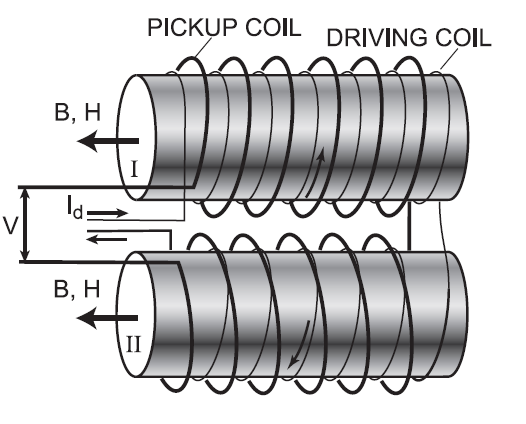
\includegraphics[width=0.50\textwidth]{schema}
\caption{Représentation d'un capteur recueillant une composante de l'espace tridimensionnel}
\end{center}
\end{figure}

L'enroulement des fils conducteurs sur les coeurs forment des bobines émettrices (chaque capteur à deux bobines émettrices). Ainsi, lorsque qu'un courant alternatif est appliqué aux fils conducteurs et que les capteurs sont positionnés dans un champ magnétique externe nul, ceux-ci émettent deux champs magnétiques (de même magnitude, mais de direction opposée, considérant l'enroulement du fil conducteur. La paire de bobine réceptrice est donc soumise à une variation de flux magnétique et la loi de Faraday nous indique que chacune de ces bobines obtient une force-électromotrice induite:
\[ \epsilon = -\frac{d \Phi}{dt} = -\frac{d}{dt} \iint_S  \vec{B}  \cdot \vec{dS}  \]  
Cependant, comme les champs magnétiques émis sont inversés et que les bobines réceptrices sont enroulées de la même façon la force-électromotrice induite totale est nulle (ne pas oublier que les capteurs sont dans un champ magnétique externe nul). Dans un autre ordre d'idée, les coeurs paramagnétiques, placées à l'intérieur des bobines émettrices, sont soumis à un champ magnétique émis variable ($\vec{H}$), ainsi les dipôles magnétiques à l'intérieur de ce matériau paramagnétique s'aligne avec la direction du champ magnétique ($\vec{H}$). Macroscopiquement, il y a présence d'une densité de flux variable ($\vec{B}$), à l'intérieur des coeurs, induit par le champ magnétique ($\vec{H}$). La relation graphique entre le champ magnétique $\vec{H}$ émis par les bobines et la densité de flux $\vec{B}$ à l'intérieur des coeurs est appelé une courbe d'hystérésis (voir figure x+1).  
  
\begin{figure}[h]
\begin{center}
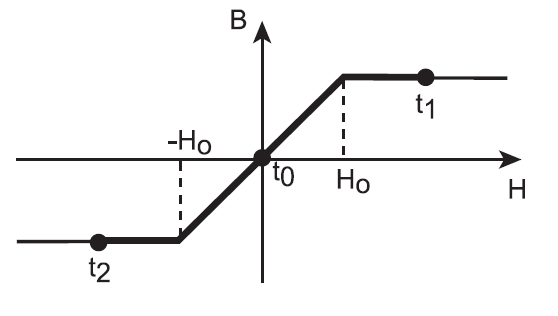
\includegraphics[width=0.50\textwidth]{hysteresis}
\caption{Courbe d'hystérésis idéalisée d'un matériau paramagnétique. Les domaines linéaires et constants sont symmétriques par rapport à l'origine.}
\end{center}
\end{figure}  

On pose l'hypothèse que le régime linéaire se situe entre $-H_o$ et $H_o$, puis que $||-H_o||=||H_o||$. Physiquement, les valeurs de $-H_o$ et $H_o$ sont  les valeurs de champ magnétique qui saturent l'aimantation des coeurs. Ainsi, lorsque l'on sort du régime linéaire $[-H_o;H_o]$, la densité de flux $\vec{B}$ est approximativement constante. Afin de bien représenter la force électromotrice induite, la loi de Faraday nous propose de trouver une représentation de $\vec{B}$ en fonction du temps. Jusqu'à présent, nous savons que $\vec{B} = \vec{B}(\vec{H}(t)) $. Cependant, chaque capteur travaille avec une composante de ces vecteurs, alors pour le besoin de la cause nous travaillerons avec les composantes de $\vec{B}$, telles que $B_i = B_i(H_i(t)$. Alors nous aurons trois composantes de force électromotrice induite:
\begin{equation}
\epsilon_i(t) = - \iint_S  \frac{\partial B_i(t)}{\partial dt}{dS_i}= -\pi r^2 \frac{\partial B_i(t)}{\partial t}   ,\ pour \ i=x,y,z 
\end{equation}
Par la suite, puisque $H_i(t)$ est produit à partir des bobines émettrices, cela  
nous permet d'avoir un certain contrôle sur la forme temporelle de $H_i(t)$ en fonction du temps, où $H_i(t)$ est péridique dans le temps, car la forme de $H_i(t)$ dépend directement de la forme d'onde du courant électrique injecté dans les bobines émettrices.
Après tout, nous voulons représenter $B_i(H_i(t))$, il faut donc combiner la fonction de $H_i(t)$ dans le temps et la courbe d'hystérésis qui met en relation $B_i$ et $H_i$. Il faut tout d'abord comprendre que le cycle d'héstérésis est parcouru entre les points $t_1$ à $t_2$ périodiquement. Comme $(B_i)$ est linéaire avec $(H_i)$ pour $[-H_o;H_o]$, les représentations graphique entre $B_i(t)$ et $H_i(t)$ dans le temps auront la même forme.  Par contre, lorsque l'on sort de la plage de linéarité $B_i(H(t))$ est approximativement une constante, ce qui veut dire que $H_i(t)$ peut continuer à varier dans le temps, lorsque $B_i(H(t))$ sature. Pour les besoins de l'explication, nous allons supposer que notre $H_i(t)$ est un signal triangulaire périodique. On peut alors bien visualiser la saturation de $B_i(t)$ à l'aide de la figure x+y.




\begin{figure}[h]
\begin{center}
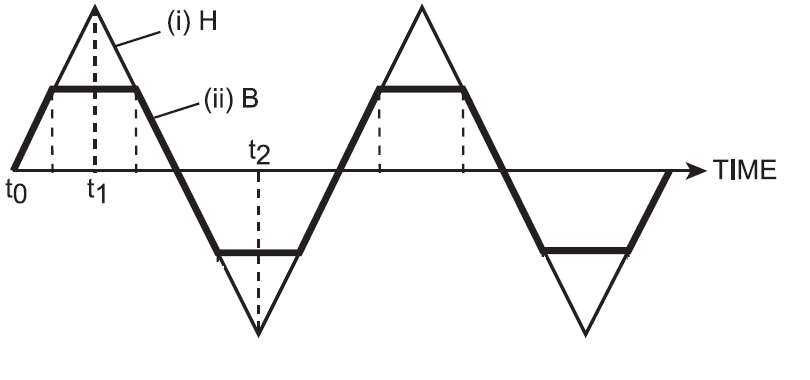
\includegraphics[width=0.50\textwidth]{saturation}
\caption{Représentation temporelle de $H_i(t)$ et de $B_i(t)$ dans le temps pour une onde de $H_i(t)$ triangulaire. On peut aussi implicitement visualiser la saturation de $B_i(t)$ les plages non-linéaires de la courbe d'hystérésis}
\end{center}
\end{figure} 




Dans l'exemple, les plages linéaires de la courbe d'hystérésis implique que le voltage induit est une constante, car $\frac{\partial B_i(t)}{\partial t} = c, \ $ et pour les plages saturées, le voltage induit est nul, car $\frac{\partial \vec{B}}{\partial t} = 0$. Ainsi, on peut s'attendre à avoir un signal périodique approximativement carré pour une bobine réceptrice. Comme les deux coeurs ont une densité de flux opposées, le voltage induit total est nul, car les deux signaux périodiques s'annulent (voir figure x+2). 

\begin{figure}[H]
\begin{center}
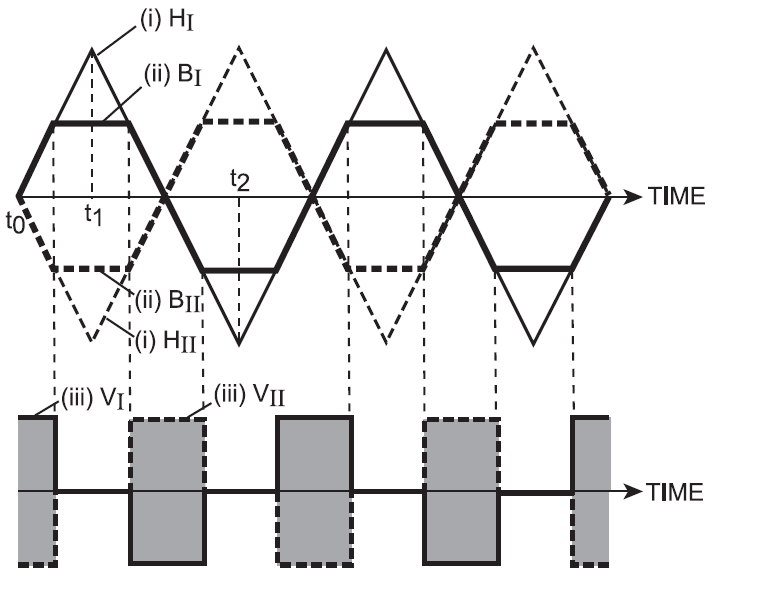
\includegraphics[width=0.50\textwidth]{voltage1}
\caption{$B_I$ représente le flux magnétique du premier coeur et $B_{II}$ le flux du second coeur. Comme les flux magnétiques sont opposés et que les bobines réceptrices sont du même sens, on retrouve un voltage induit nul.}
\end{center}
\end{figure} 

Notre voltage nul, tel que décrit ci-dessus est notre configuration de référence pour un champ externe nul. Pour obtenir cette configuration, il peut être nécessaire de placer le système dans une cage de Faraday, afin d'éviter que la mesure de référence soit perturbée par des facteurs externes non-voulues. Ensuite, en positionnant notre système activé (courant électrique alternatif) dans un champ magnétique externe constant, le cycle d'hystérésis n'est plus parcourue de manière symmétrique. La position moyenne du cycle n'est plus à l'origine, mais à un point $H_{ext}$ (voir figure 5), ce qui fait que les voltages induits sont translatés par rapport à la configuration nulle. En faisant des voltages induits dans les deux bobines réceptrices, on retrouve un voltage résiduel (voir figure).

\begin{figure}[H]
\begin{center}
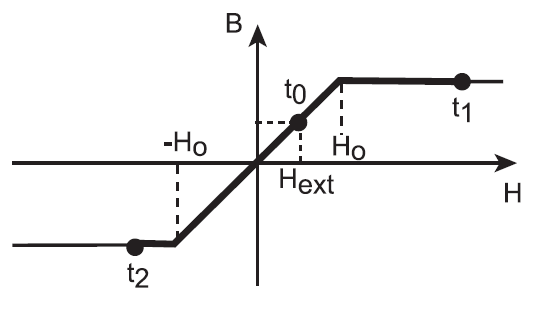
\includegraphics[width=0.50\textwidth]{hysteresis2}
\caption{figure 2 blabla}

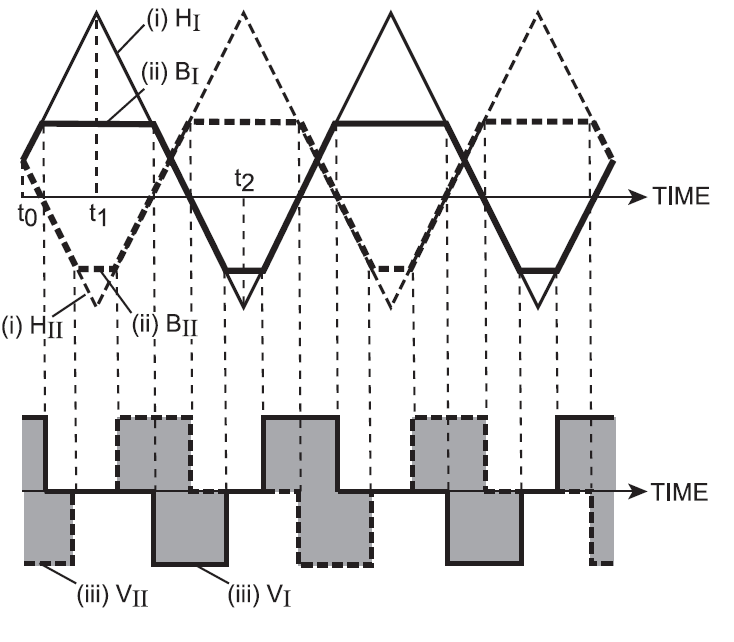
\includegraphics[width=0.50\textwidth]{voltage2}
\caption{figure 3 blabla}
\end{center}
\end{figure} 

Ce voltage induit résiduel additionné est proportionnel au champ magnétique externe (mettre référence). RAJOUTER BLABLA



\end{document}